% This is samplepaper.tex, a sample chapter demonstrating the
% LLNCS macro package for Springer Computer Science proceedings;
% Version 2.20 of 2017/10/04
%
\documentclass[runningheads]{llncs}
%
\usepackage{todonotes}
\usepackage{amsmath}
\usepackage{booktabs} % For pretty tables
\usepackage{caption} % For caption spacing
\usepackage{subcaption} % For sub-figures
\usepackage{graphicx}
\usepackage[all]{nowidow}
\usepackage[utf8]{inputenc}
\usepackage{tikz}
\usepackage{multicol}
%\usepackage{algpseudocode,algorithm,algorithmicx}
%\usepackage{minted}
\usepackage[ruled,linesnumbered,algochapter]{algorithm2e} % Enables the writing of pseudo code.
\usepackage[hidelinks]{hyperref}
\usepackage{cleveref}
\usepackage{amsmath}    % Extended typesetting of mathematical expression.
\usepackage{amssymb}    % Provides a multitude of mathematical symbols.
\usepackage{mathtools}  % Further extensions of mathematical typesetting.
\usepackage[inline]{enumitem} % Horizontal lists
% Used for displaying a sample figure. If possible, figure files should
% be included in EPS format.
%
% If you use the hyperref package, please uncomment the following line
% to display URLs in blue roman font according to Springer's eBook style:
% \renewcommand\UrlFont{\color{blue}\rmfamily}

\usepackage{subcaption}

\newcommand{\card}[1]{\left\vert{#1}\right\vert}
\newcommand*\Let[2]{\State #1 $\gets$ #2}
\definecolor{blue}{HTML}{1F77B4}
\definecolor{orange}{HTML}{FF7F0E}
\definecolor{green}{HTML}{2CA02C}


\renewcommand{\topfraction}{0.85}
\renewcommand{\bottomfraction}{0.85}
\renewcommand{\textfraction}{0.15}
\renewcommand{\floatpagefraction}{0.8}
\renewcommand{\textfraction}{0.1}
\setlength{\floatsep}{3pt plus 1pt minus 1pt}
\setlength{\textfloatsep}{3pt plus 1pt minus 1pt}
\setlength{\intextsep}{3pt plus 1pt minus 1pt}
\setlength{\abovecaptionskip}{2pt plus 1pt minus 1pt}

\begin{document}
%
\title{A Correlation-Preserving Fingerprinting Technique for Categorical Data\\ in Relational Databases}
%
%\titlerunning{Abbreviated paper title}
% If the paper title is too long for the running head, you can set
% an abbreviated paper title here
%
\author{Tanja Sarcevic\inst{1}\orcidID{0000-0003-0896-9193} \and
Rudolf Mayer\inst{1}\orcidID{0000-0003-0424-5999}}
%
%\authorrunning{F. Author et al.}
% First names are abbreviated in the running head.
% If there are more than two authors, 'et al.' is used.
%
\institute{SBA Research, Vienna, Austria\\
\email{\{TSarcevic,RMayer\}@sba-research.org}\\}
%
\maketitle              % typeset the header of the contribution
%
\begin{abstract}
Fingerprinting is a method of embedding a traceable mark into digital data, to verify the owner and identify the recipient a certain copy of a data set has been released to.
This is crucial when releasing data to third parties, especially if it involves a fee, or if the data is of sensitive nature, due to which further sharing and leaks should be discouraged and deterred from.
Fingerprinting and watermarking are well explored in the domain of multimedia content, such as images, video, or audio.

The domain of relational databases is explored specifically for numerical data types, for which most state-of-art techniques are designed.
However, many datasets also, or even exclusively, contain categorical data.

We, therefore, propose a novel approach for fingerprinting categorical type of data, focusing on preserving the semantic relations between attributes, and thus limiting the perceptibility of marks, and the effects of the fingerprinting on the data quality and utility.
We evaluate the utility, especially for machine learning tasks, as well as the robustness of the fingerprinting scheme, by experiments on benchmark data sets.

\keywords{Fingerprinting \and Relational Database \and Categorical Data \and Data Utility Analysis \and Robustness Analysis}

\end{abstract}
%
%
%
\section{Introduction}\label{sec:intro}
\textit{Digital watermarking} is a method that helps protecting intellectual property for various types of  data. It embeds a piece of information into the data to provide an identification of the data owner.
Since it does not control access to data, watermarking is a \textit{passive} protection tool.
Applications include copyright protection, fraud or tamper detection.
\textit{Fingerprinting} is used for data leakage source tracking.
It is a special application of watermarking, where different recipients of the data obtain differently watermarked content.
This property allows identifying the authorised recipient of the information.
First techniques were developed for the multimedia domain (images, audio, video). 
The generally large amount of data required to represent this content offers space to embed the marks, without significantly affecting the actual content.
The application domain was later extended to other types of digital data such as text, software, or relational databases.
The effects caused by marking this type of data is a bigger concern. 

In the domain of fingerprinting relational data, most state-of-the-art techniques address only numerical type of data.
It is important to address the problem of fingerprinting categorical values, as  many real world datasets contain some or exclusively categorical attributes. 
Limitations are the discrete nature of categorical values, where the required modifications for embedding the marks cause a discrete (and not minor) alteration, as well as mutual correlations between attributes.
Therefore, any change to the categorical value is more perceptible than a (minor) change to the numerical.

Our approach addresses the problem of semantic relations between categorical attributes in a relational database that can be disturbed by fingerprinting. 
Considering attributes independently of each other and embedding a random mark into a categorical value might lead to non-consistent records, by introducing an uncommon or impossible combination of values in the data. 
For example, in a database containing attributes such as \textit{sex} and \textit{numberOfPregnancies}, these attributes intuitively contain an impossible combination of values: (\textit{sex}:male, \textit{numberOfPregnancies}:1).
A very uncommon combination of values could be in a medical database containing information about the patients suffering from Alzheimer's disease: 
(\textit{alzheimersStage}:middle, \textit{employed}:yes), but this might be introduced by a random fingerprint mark.
With database domain knowledge, these examples would be rather suspicious and thus perceptible. 
In our approach, we therefore aim to take into account the correlation between the values of different attributes and avoid uncommon combinations. 

The remainder of this paper is organised as follows. In \Cref{sec:related-work} we describe the related work in the area of watermarking and fingerprinting relational databases.
In \Cref{sec:scheme} we describe our scheme for fingerprinting categorical attributes. In \Cref{sec:evaluation} we present the analysis of the scheme's robustness against malicious attacks and data utility. We provide conclusions in \Cref{sec:conclusion&future-work}.

\section{Related work}\label{sec:related-work}

%\paragraph{Watermarking}
The technique pioneering \textbf{watermarking relational data} by Agrawal et al. \cite{agrawal2003watermarking} allows watermarking datasets containing numerical data.
Minor alterations to the data are made in specific positions, creating a pseudo-random pattern. If the pattern is known, it is possible to extract the watermark from the data, and thus prove the ownership.
The technique relies on a key property of one-way hash functions -- it is easy to calculate an output (hash value) for a given input, but computationally difficult to do the inverse.
This means that only by knowing the key that was used in the embedding process of watermarking (which is kept by the owner of data), one can extract the watermark from the data.
The technique has been extended in later approaches. They differ by the patterns of embedding the watermark, or the type of information used as a watermark.
For instance, a watermark in a form of a binary image \cite{wang2008atbam}, owner’s speech compressed and converted into a bit-stream as watermark information \cite{wang2008speech}, etc.

Categorical data types require different techniques for watermarking purposes than numerical ones, due to their discrete nature.
This is a major the reason for considerably fewer watermarking and fingerprinting techniques proposed for categorical data types. 
Sion et al. \cite{sion2004proving} propose a watermarking scheme for categorical data in relational databases, and later extend it \cite{sion2004rights}.
The scheme in its simplest form applies a pseudo-random mark to the categorical value based on the primary key of the relation by changing it to another value from the attribute domain.
The authors further address the malicious attack of vertical data partitioning where even the primary key is potentially removed.
The extended version of the scheme applies a pseudo-random mark to the categorical value based on other categorical values from the relation and repeats the process for every pair of categorical attributes in the dataset.
It utilises correlation and discreteness of the categorical attributes as a strength to avoid the scheme’s dependence on the primary key, instead of it being a weakness in terms of lack of data redundancy for mark embedding.
However, the scheme quickly gets too complex for dataset with many categorical attributes.
Furthermore, it does not address semantic correlation between categorical attributes.

One of the earliest \textbf{fingerprinting} schemes for relational data \cite{li2005fingerprinting} is based on Agrawal et al. \cite{agrawal2003watermarking}.
Other fingerprinting schemes propose different patterns for marking the data. In \cite{liu2004block}, the owner’s unique fingerprinting is embedded into previously partitioned blocks of data.
In \cite{guo2006fingerprinting} the fingerprint is embedded in two-layers - the first of which identifies the owner. Once the verification is successful, the recipient can be detected from the second layer.
The watermarking and fingerprinting system Watermill \cite{lafaye_watermill:_2008} extends the methods by considering the constraints of data alteration and treating fingerprinting as an optimisation problem.

Fingerprinting techniques for categorical data are less researched, compared to techniques for numerical.
The fingerprinting technique from \cite{Kieseberg2014fingerprinting} can be applied on relational database containing any type of data.
It exploits the fact that different sets of equivalence classes can be created in the data when making it k-anonymous \cite{sweeney2002k}.% -- each fingerprint is created by obtaining a slightly different set of equivalence classes.
However, the scheme has several limitations, such as a limited number of available fingerprints, diverging utility of different fingerprinted data copies and needing to keep each recipient’s fingerprint in a separate data storage which associates additional security risk. 
In our previous work \cite{sarcevic19_fingerprinting}, we introduced a simplistic scheme for fingerprinting categorical values. 
In this approach, all categorical values are firstly encoded to numerical. 
The scheme for fingerprinting numerical values from \cite{li2005fingerprinting} is then applied to the dataset, and the values are decoded back to categorical. 
This scheme is essentially altering a categorical value to a random one from the domain of the attribute. 
One limitation is that the scheme does not consider any relation between the attributes of the dataset. However, the scheme may serve as a robust solution for fingerprinting datasets with semantically independent and non-highly correlated attributes.

All the above schemes claim to satisfy the \textit{blindness} property -- the original dataset is not needed for the successful watermark/fingerprint extraction. 

\section{Fingerprinting categorical data}\label{sec:scheme}
Fingerprinting consists of two main processes: \textit{insertion (embedding)} and \textit{detection (extraction)}.
The insertion process comprises fingerprint creation and embedding to the data.
It embeds a different mark for each distributed copy, specific for each recipient.
The output is the marked copy of the data that can be distributed.
The detection process extracts the fingerprint from the data.
It reports the existence of a fingerprint in the data given as the input, and identifies the recipient.
We describe these two processes in detail below for our proposed scheme.

\subsection{Prerequisites and notation}
A \textit{Cryptographic Hash function} is a deterministic function that takes a string input of any length and returns a fixed-size string value called \textit{hash value}. A hash function has three main properties: (i) it is easy to calculate a hash value for any given input string, (ii) it is computationally difficult to calculate an input that has given a certain hash value and (iii) it is extremely unlikely that two different inputs, even remotely different, have the same hash value.
\paragraph A \textit{Pseudo-random number sequence generator (PRNG)} is an algorithm for generating a sequence of numbers whose properties approximate the properties of sequences of random numbers. The PRNG-generated sequence is not truly random, because it is completely determined by an initial value, called the \textit{seed}.
\paragraph{k-nearest neighbours algorithm (k-NN)} is a method that (in classification task) classifies the object by a plurality vote of its neighbours, with the object being assigned to the class most common among its $k$ nearest neighbours. 
The neighbourhood of an object can be determined in multiple ways,  frequently for discrete variables a form of the \textit{Hamming distance} (overlapping measure) is used.
We use an adaptation of k-NN with Hamming distance as a step in the insertion algorithm. k-NN is, as well, used as one of the classifiers for our data utility analysis in \Cref{sec:utility}.
\begin{table}
\centering
\caption{The notions of the most common parameters and functions}
\label{table:notation}
\begin{tabular}{@{}c|c@{}}
\toprule
 Notation & Meaning \\ 
 \midrule
 $\mathcal{R}$ & database relation \\
 \textit{P} & primary key attribute \\
 $A_i$ & $i^{th}$attribute \\
 \textit{v} & number of attributes \\
 $N$ & number of tuples  \\
  \bottomrule 
\end{tabular}
\begin{tabular}{@{}c|c@{}}
     \toprule
 Notation & Meaning \\ 
 \midrule
 $\mathcal{K}$ & owner's secret key  \\ 
 $1/\gamma$ & ratio of tuples to be marked\\
 \textit{L} & length of a fingerprint \\
 $|$ & concatenation function \\
 $\mathcal{H}$ & hash function \\
 \bottomrule
\end{tabular}
\end{table}


\subsection{Insertion}\label{subsec:insertion}
The insertion algorithm introduces modifications to the original data on the pseudo-randomly selected positions in the dataset.
The main outline of the algorithm is modelled on the fingerprinting algorithm from \cite{li2005fingerprinting}. Namely, the legitimate owner of the data holds her secret key which is used to verify the ownership of the data and detect the potential malicious users.
For each data user that is authorised to use the fingerprinted data (recipient), a distinct fingerprint is generated. The fingerprint defines the pattern of applying the modifications on the data, and ultimately, this pattern identifies the specific data recipient.
 
The insertion algorithm is designed with the aim of preserving the correlations between categorical attributes in a relational database.
This is resulting in zero occurrences of value combinations that were not initially in the original database, and low frequency occurrences of value combinations that were already rare in the original database.
This insertion algorithm reduces perceptibility of a fingerprint mark in a relational database.


\begin{algorithm}
  \KwIn{database $\mathcal{R}$ with scheme $(P, A_{0}, ..., A_{v-1})$, buyer $n$'s ID $id$}
  \KwOut{fingerprinted database $\mathcal{R'}$}
  fingerprint of buyer $n$: $\mathcal{F}(\mathcal{K},id)=\mathcal{H}(\mathcal{K}|id)$
  \\
  \ForEach{tuple $r \in \mathcal{R}$}
  {
    \If{$(\mathcal{S}_{1}(\mathcal{K}|r.P)$ mod $\gamma == 0)$}{
        attribute\_index $i = \mathcal{S}_2(\mathcal{K}|r.P)$ mod $v$
        \\
        fingerprint\_index $l=\mathcal{S}_3(\mathcal{K}|r.P)$ mod $L$
        \\
        fingerprint\_bit $f=f_l$\\
        mask\_bit $x=0$ if $\mathcal{S}_4(\mathcal{K}|r.P)$ is even; $x=1$ otherwise \\
        mark\_bit $m=x \oplus f$ \\
        \uIf{m == 1}{
            neighbourhood = $select\_neighbours()$ \\
            target\_values, freq = $get\_frequencies(\text{neighbourhood})$\\
            $r.A_i = random(\text{target\_values}, weight=\text{freq})$
        }
        \uElse{no marking}
    }
    
  }
  \Return{$\mathcal{R'}$}
  \caption{Insertion}
  \label{alg:insertion}
\end{algorithm}

\paragraph{}
The insertion algorithm of our fingerprinting scheme is shown in \Cref{alg:insertion}.
The algorithm starts with creating a distinct fingerprint for an authorised data receiver.
A user's fingerprint $\mathcal{F}$ is a bit-string of length $L$ generated as a hash value of the owner's secret key $\mathcal{K}$ and user's identification $id$ (which may be available publicly). 

In lines 2-15 of \Cref{alg:insertion}, the fingerprint is embedded in the data. 
For each tuple (row) $r$ in the database $\mathcal{R}$, a pseudo-random number sequence generator $\mathcal{S}$ is seeded with a concatenation of the owner's secret key $\mathcal{K}$ and the primary key of the tuple, $r.P$. 
This step allows the creation of a distinct sequence of numbers for each of the database's tuples. 
Furthermore, seeding the generator with the owner's secret key ensures that the sequence cannot be generated without knowing the secret key. 
Using the modulo value of the first number from the pseudo-random sequence with the parameter $\gamma$, the algorithm decides if the observed tuple is selected for introducing a modification (line 3). 
Due to the uniform distribution of the output of a pseudo-random sequence generator, approximately $N/\gamma$ tuples will be selected for marking. 
Therefore, with parameter $\gamma$, we control the amount of modifications in a fingerprinted copy of the data. 
In the line 4, the next pseudo-random number is generated, which is used to select the attribute $A_i$ for marking.
In lines 5--6, the next pseudo-random number from the sequence is used to select the fingerprint bit $f_l$ that will mark the value $r.A_i$. 
The purpose of lines 7 and 8 is to obtain a uniform distribution of marks that are modifying the data. 
We can see in lines 9-14 that the marking is performed only if the mark value is 1. 
If fingerprint bits are directly used as marking bits, they can heavily influence the amount of modifications in the data, as it is not expected that ones and zeroes will be equally represented in a fingerprint.
Fingerprint bits are, thus, subjected to an $xor$ function with uniformly distributed mask bits $x$, in the line 8.
Finally, if the mark value is 1, the data value is modified. 

In the process of marking the data we do not only consider the value $r.A_i$ selected for marking, but the entire tuple $r$. 
The goal is to modify the value $r.A_i$ to a value that is \textit{likely to occur in the original database}, considering the other values of the same tuple. 
To achieve this, the algorithm searches in the database for the tuples most similar to the one observed, i.e the most similar "neighbours" (cf. line 10).
Once the neighbours are selected, the algorithm extracts the values of the attribute $A_i$ from the neighbouring tuples, $target\_values$, and calculates their frequencies (line 11).
The value $r.A_i$ will be changed to one of the values appearing in the attribute $A_i$ of the neighbourhood. The calculated frequencies of these values correspond to the probability for a specific value being selected.
The line 12 shows the selection of the new value: it is randomly chosen from the neighbourhood values, weighted by the frequency of their occurrences. 
This technique is known in genetic algorithms as a fitness proportionate selection, or roulette wheel selection, a genetic operator used for selecting potentially useful solutions for recombination.
The analogy to a roulette wheel can be drawn as follows: each candidate value represents a pocket on the roulette wheel; the size of the pockets are proportionate to the frequency of the values among the neighbours.
Thus, the most common value is the most likely to be drawn, but any value with a non-zero frequency can be chosen.

Once all the tuples are examined, the output of the algorithm is a fingerprinted copy of the data, $\mathcal{R'}$.

\subsection{Detection}
The detection algorithm extracts a fingerprint from a fingerprinted copy of the data by searching for the specific pattern embedded by the insertion algorithm. 
The pseudo-code for the detection algorithm is shown in \Cref{alg:detection}.

\begin{algorithm}
  \KwIn{fingerprinted database $\mathcal{R'}$ with scheme $(P, A_0, ..., A_{v-1})$, original database $\mathcal{R}$ with scheme $(P,A_0,...,A_{v-1})$}
  \KwOut{suspected buyer's ID $id$}
  fingerprint template $\mathcal{F}=(f_0,...,f_{L-1})=(?,...,?)$  \\
  $count[i][0]=count[i][1]=0$ \textbf{for} $i=0$ to $L-1$\\ 
  \ForEach{tuple $r \in R'$}
  {
    \If{$\mathcal{S}_1(\mathcal{K},r.P)$ mod $\gamma==0$}
    {
        attribute\_index $i=\mathcal{S}_2(\mathcal{K},r.P)$ mod $v$\\
        fingerprint\_index $l=\mathcal{S}_3(\mathcal{K},r.P)$ mod $L$\\
        mask\_bit $x=0$ if $\mathcal{S}_4(\mathcal{K},r.P)$ is even; $x=1$ otherwise\\
        \uIf{$r.A_i$ is different from the original}{
            mark\_bit $m = 1$
        }
        \uElse{
            mark\_bit $m= 0$
        }
        
        fingerprint\_bit $f=m \oplus x$\\
        $count[l][f]++$ 
    }
  }
  //recover the fingerprint\\
  \For{$l=0$ to $L-1$}
  {
    \If{$count[l][0]+count[l][1]==0$}
    {
        \Return{\textit{none suspected}}
    }
    $f_l=0$ if $count[l][0]/(count[l][0]+count[l][1])>\tau$\\
    $f_l=1$ if $count[l][1]/(count[l][0]+count[l][1])>\tau$\\
    \Return{\textit{none suspected}} otherwise
  }
  $\mathcal{F}=(f_0,...,f_{L-1})$\\
  $id=detect(\mathcal{F}$\\
  \uIf{$id\geq0$}
  {
    \Return{$id$}
  }
  \Else
  {
    \Return{\textit{none suspected}}
  }
  \caption{Detection}
  \label{alg:detection}
\end{algorithm}

Each fingerprint bit might be embedded multiple times in the data, so the detection algorithm searches for all the occurrences and counts the detected values.
The algorithm starts by initialising the empty fingerprint template of length $L$, and the votes for fingerprint bit values, all set to zero. 
The next step is to find the tuples and attributes that should have been fingerprinting according to the pseudo-random number sequence (lines 3-5). 
Note that the concatenation of the owner's secret key and dataset primary key values is used as a seed to generate exactly the same number sequences as in the insertion algorithm. 
We retrieve the fingerprint bit index $l$ and the mask bit $x$ in the same manner (lines 6 and 7).
Next, to find the value of the mask bit $m$, it is necessary to compare the suspected fingerprinted database to the original. 
If the corresponding value is different from the original, meaning it was modified by the insertion algorithm, then the value $m$ was 1 in the insertion algorithm, otherwise 0. 
This step is performed in the lines 8-11.
In line 12, we obtain the fingerprint bit value $f$ from the mark bit $m$ and mask bit $x$\footnote{If $m=x \oplus f$, then $f=m \oplus x$}.
The line 13 represents the vote that the fingerprint bit on position $l$ is value $f$.

After all votes are collected, the algorithm attempts to recover the fingerprint.
In case the votes for some fingerprint bit on position $l$ do not exist (all remained zero), then the fingerprint can not be recovered and it is not possible to identify the authorised user who owns the given fingerprinted copy (lines 18-20).
Otherwise, the value for every fingerprint bit is decided by a \textit{majority voting}, i.e. the most frequent value is chosen.
The quorum for the majority can, besides the simple absolute majority described above, also be a user-specified setting, with the parameter $\tau\in[0.5,1)$, i.e. a larger consensus among the votes can be required.

The extracted fingerprint template is compared to fingerprints of authorised recipients of the data (cf. line 26 in \Cref{alg:detection}).
In case of a perfect match, a user is identified.

\subsection{Discussion}
In the \Cref{subsec:insertion} we propose an insertion algorithm that can be applied to categorical attributes in the relational data and keep it as the main focus of the study. 
Indeed, the insertion algorithm, \Cref{alg:insertion}, assumes a database $\mathcal{R}$ with attributes $A_0,...A_{v-1}$ of a only categorical variables as its input.
Following our claims from above, real-world databases are oftentimes containing attributes of various data types. 
For the purpose of fingerprinting such databases, one may select either numerical or categorical attributes, depending on what makes the majority and apply a corresponding fingerprinting scheme, as one solution. 
The other solution would be to combine schemes for each data type and perform them separately. This way, all of the attributes may be selected for marking, and therefore harder to attack compared to the first solution. 
On the other hand, dealing with multiple secret keys and parameters in the fingerprinting process might not be convenient for a practical use. 

The proposed scheme relies on the existence of database's primary key attribute. 
Li et. al. \cite{li2005fingerprinting} proposed a technique for creating a virtual primary key for relational databases in case one does not exist in the original database.

In the data marking phase of \Cref{alg:insertion}, we need to select the neighbourhood of the observed tuple. 
We find the neighbours using the nearest neighbours algorithm with a form of the Hamming distance and let the user define the parameter $k$ and the attributes that will be included in calculating the nearest neighbours.

\paragraph{}
Due to the requirement to preserve semantic relations in the fingerprinted copy of the dataset, the modified values are calculated from the data itself, instead of some external deterministic method. 
As a result, for fingerprint extraction, it is necessary to have access to the original dataset (line 8 of \Cref{alg:detection}). Therefore, our scheme is a \textit{non-blind} scheme. 

\section{Evaluation}\label{sec:evaluation}
For our experiments, we choose two datasets from the UCI Machine Learning repository\footnote{http://archive.ics.uci.edu/ml} that feature categorical data: Breast Cancer\footnote{\url{https://archive.ics.uci.edu/ml/datasets/breast+cancer}} and Nursery\footnote{\url{https://archive.ics.uci.edu/ml/datasets/nursery}}.
The Breast Cancer dataset describes breast cancer features and whether or not the cancer reoccurred. The dataset has ten columns (including the target attribute) and 286 rows. 
The Nursery dataset contains data for ranking applications for nursery schools. It contains 12,980 rows and nine columns (including the target attribute).
In this section we present our analyses on the scheme's robustness and the utility of the fingerprinted data.

\subsection{Attacks and Robustness Analysis} \label{sec:robustness}
Fingerprinting techniques are vulnerable to operations that potentially erase the fingerprint from the database.
These operations can be either a result of benign updates of the database, or malicious attacks by an adversary. 
In either case, a fingerprint should be robust enough to be recognisable by the owner even from the altered data.

For our evaluation of the scheme for categorical data, we consider the following attacks on the fingerprinted database:
\begin{itemize}
    \item \textbf{Subset attack}: The attacker releases only a subset of the fingerprinted database.
    We differentiate two cases:
    In a \textbf{horizontal} attack, a subset of complete tuples (rows) is removed from the original copy of the dataset.
    In a \textbf{vertical} attack, one or more columns are removed from the database. 
    \item \textbf{Flipping attack}: The attacker flips a selected value to a random, valid one, and repeats this for multiple data values.
    This attack is the adapted version of the \textit{bit-flipping attack} from the domain of fingerprinting numerical values, where the attacker flips a least significant bit of a chosen set of values.
\end{itemize}

In the following, we present our empirical evaluation of the robustness of the proposed fingerprinting techniques against the attacks described above. We use the following robustness measures \cite{li2005fingerprinting} in our experiments: 
\begin{itemize}
  \item \textbf{Misattribution false hit} $(fh^A)$: The probability of \textit{detection of an incorrect}, but existing fingerprint from fingerprinted data.
  \item \textbf{False negative} $(fn)$: The probability of \textit{not detecting} a valid fingerprint from fingerprinted data.
  \item \textbf{False miss} $(fm)$: The probability of failing to detect an embedded fingerprint correctly. False miss rate is the sum of the false negative and misattribution false hit rates, i.e. $fm=fh^A+ fn$.
\end{itemize}

%\subsubsection{Experiments}

In our scheme for fingerprinting categorical data, the exact positions of fingerprint marks are known only with the knowledge of the owner's secret key. 
Assuming the key being protected, we thus model the attacker such that her choice of positions within the database to attack is random. 
We further assume the attacker knows the algorithmic steps of insertion and detection processes, and its parameters -- in fact, the only unknown is the owner's secret key. 

We choose the values for $\gamma$ for the Breast Cancer dataset: (1, 2, 3, 5) and length of fingerprints is $L=8$. Parameter $\gamma$ is expected to contribute the most to the robustness level of the scheme, since it defines the number of fingerprint marks in the data. 
For the Nursery dataset, due to its bigger size, we experiment with the larger values for $\gamma$: (5, 10, 20, 30). The length of the fingerprint is set to $L=64$. 

\paragraph{Horizontal Subset Attack}

% old figures, separated
% \begin{figure}
%     \centering
%     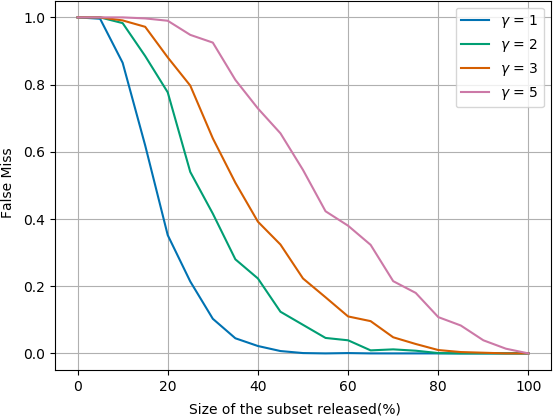
\includegraphics[width=0.75\textwidth]{figures/horizontal_subset_bc.png}
%     \caption{Robustness against horizontal subset attack on Breast Cancer data}
%     \label{fig:horizontal-subset-bc}
% \end{figure}
% \begin{figure}
%     \centering
%     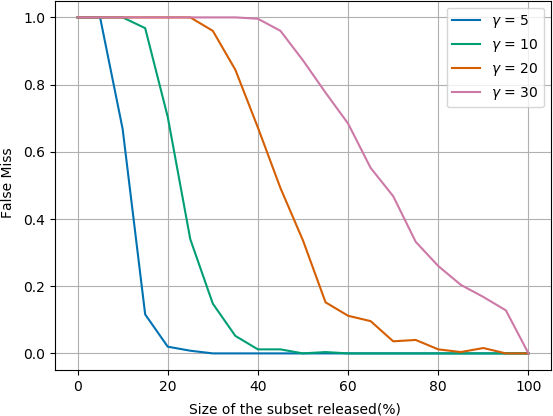
\includegraphics[width=0.75\textwidth]{figures/horizontal_subset_n.png}
%     \caption{Robustness against horizontal subset attack on Nursery data}
%     \label{fig:horizontal-subset-n}
% \end{figure}

% new figure, side-by-side
\begin{figure*}[th]
    \centering
    \begin{subfigure}{.42\textwidth}
        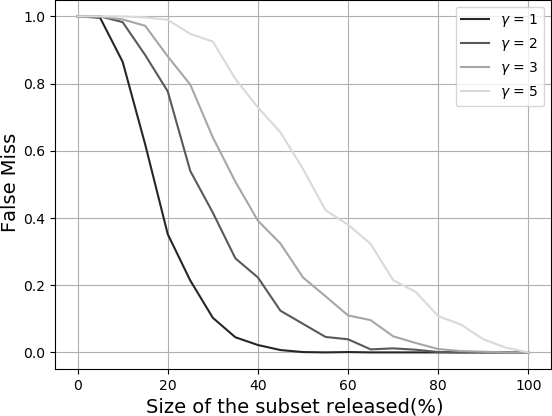
\includegraphics[width=1\linewidth]{figures/horizontal_subset_bc_grey.png}
        \caption{Breast Cancer dataset}
        \label{fig:horizontal-subset-bc}
    \end{subfigure}
    \hspace{0.02\textwidth}
    \begin{subfigure}{.42\textwidth}
        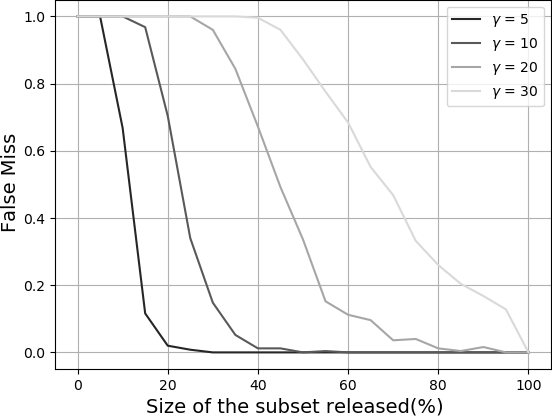
\includegraphics[width=1\linewidth]{figures/horizontal_subset_n_grey.png}
        \caption{Nursery dataset}
        \label{fig:horizontal-subset-n}
    \end{subfigure}
    \caption{Robustness against horizontal subset attack}
    \label{fig:horizontal-subset}
\end{figure*}


We simulate the horizontal subset attack, and over a number of runs measure the attacker's success via the False Miss rate depending on the amount of data she chooses to publish.
%\Cref{fig:horizontal-subset-bc} and \Cref{fig:horizontal-subset-n} show the results from the experiments with Breast Cancer data and Nursery data, respectively. 

As can be seen in \Cref{fig:horizontal-subset-bc,fig:horizontal-subset-n}, the false miss rate shows a decreasing trend for more data released.
A robust scheme should minimise the false miss rate.
Choosing smaller values for $\gamma$, i.e. more marks in the data, results in lower false miss rates.

The analysis shows the best robustness for the scheme with $\gamma=1$ (i.e. each row will be fingerprinted) for fingerprinting Breast Cancer data. The false miss rate is close to zero for approximately 40\% of published rows, i.e. the attacker needs to delete more than 60\% of the data to increase her chances of destroying a fingerprint.
Choosing the value $\gamma=5$ for the same dataset gives the attacker better chances for success.
Similar results are presented in \Cref{fig:horizontal-subset-n} for the Nursery dataset, where schemes with smaller data show better robustness. 
Interestingly, the scheme with $\gamma=5$ for Nursery dataset outperforms even the most robust scheme (the one with $\gamma=1$) for Breast Cancer data. Furthermore, it even more outperforms the scheme for Breast Cancer with the same value $\gamma=5$. 
This is because the size of the fingerprinted dataset plays an important role in the robustness of the scheme.
Fingerprinted using the same value for the parameter $\gamma$, larger dataset will count more marks than the smaller, therefore making the fingerprint harder to erase.

$fh^A$ was zero in all of the experiments, therefore the recorded $fm$ was contained of false negatives only ($fn$). 

\paragraph{Vertical subset attack}

% old figures, separated
% \begin{figure}
%     \centering
%     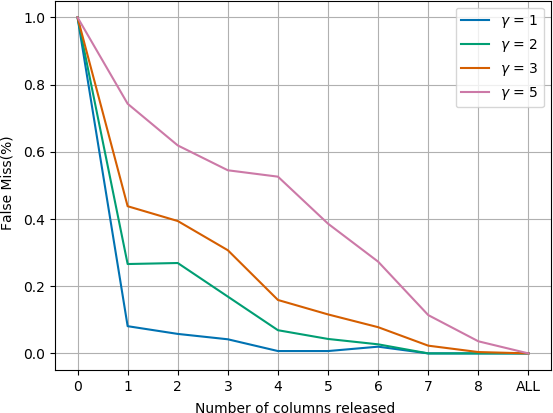
\includegraphics[width=0.75\textwidth]{figures/vertical_subset_bc.png}
%     \caption{Robustness against vertical subset attack on Breast Cancer data}
%     \label{fig:vertical-subset-bc}
% \end{figure}
% \begin{figure}
%     \centering
%     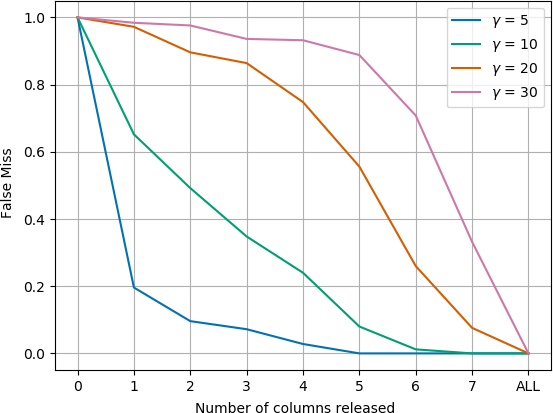
\includegraphics[width=0.75\textwidth]{figures/vertical_subset_n.png}
%     \caption{Robustness against vertical subset attack on Nursery data}
%     \label{fig:vertical-subset-n}
% \end{figure}

% new figure, side-by-side
\begin{figure*}[th]
    \centering
    \begin{subfigure}{.42\textwidth}
        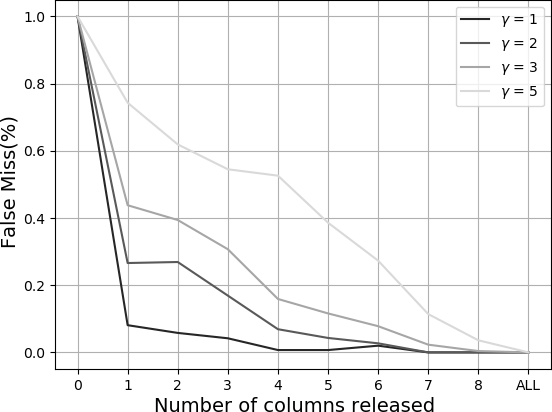
\includegraphics[width=1\linewidth]{figures/vertical_subset_bc_grey.png}
        \caption{Breast Cancer dataset}
        \label{fig:vertical-subset-bc}
    \end{subfigure}
    \hspace{0.02\textwidth}
    \begin{subfigure}{.42\textwidth}
        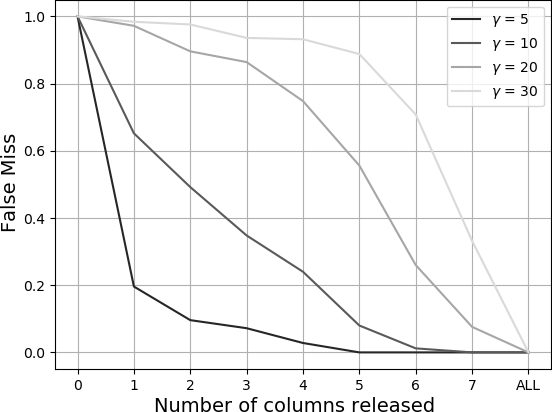
\includegraphics[width=1\linewidth]{figures/vertical_subset_n_grey.png}
        \caption{Nursery dataset}
        \label{fig:vertical-subset-n}
    \end{subfigure}
    \caption{Robustness against vertical subset attack}
    \label{fig:vertical-subset}
\end{figure*}


Datasets with few columns may be very susceptible to a vertical attack. 
The results of our analysis are shown in \Cref{fig:vertical-subset-bc,fig:vertical-subset-n} for Breast Cancer and Nursery datasets, respectively. 
The false miss rate is larger for cases where the attacker releases fewer columns. 
The most robust scheme for Breast Cancer with $\gamma=1$ shows the $fm$ of only 0.1 for only one released column.
In the \Cref{fig:vertical-subset-n}, the trend of decrease of the false miss rate is slower than in the previous case due to fewer columns in the Nursery data. Erasing one column in the Nursery data shows more negative effect on robustness than erasing a column in the Breast Cancer dataset.  
%
$fh^A$ was zero in all of the experiments.

\paragraph{Flipping attack}
% old figures, separated
% % Breast Cancer database
% \begin{figure}
%     \centering
%     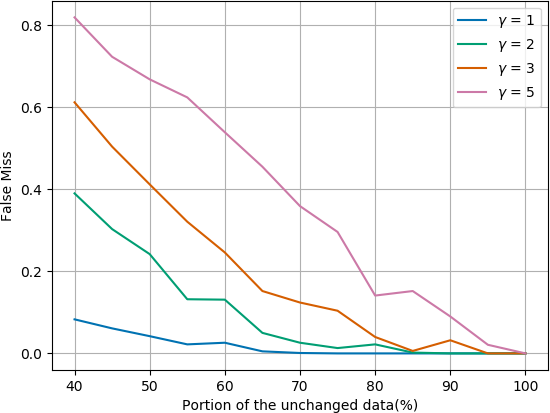
\includegraphics[width=0.75\textwidth]{figures/bit_flipping_bc.png}
%     \caption{Robustness against flipping attack on Breast Cancer data}
%     \label{fig:bit-flipping-bc}
% \end{figure}
% 
% % Nursery database
% \begin{figure}
%     \centering
%     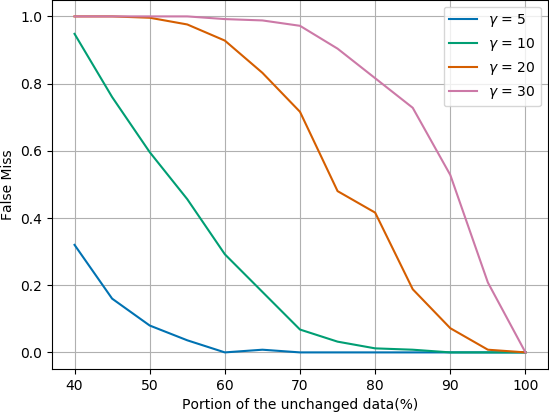
\includegraphics[width=0.75\textwidth]{figures/bit-flipping_n.png}
%     \caption{Robustness against flipping attack on Nursery data}
%     \label{fig:bit-flipping-n}
% \end{figure}


% new figure, side-by-side
\begin{figure*}[th]
    \centering
    \begin{subfigure}{.42\textwidth}
        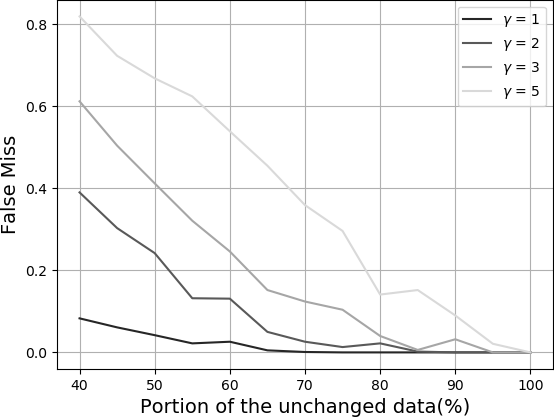
\includegraphics[width=1\linewidth]{figures/bit_flipping_bc_grey.png}
        \caption{Breast Cancer dataset}
        \label{fig:bit-flipping-bc}
    \end{subfigure}
    \hspace{0.02\textwidth}
    \begin{subfigure}{.42\textwidth}
        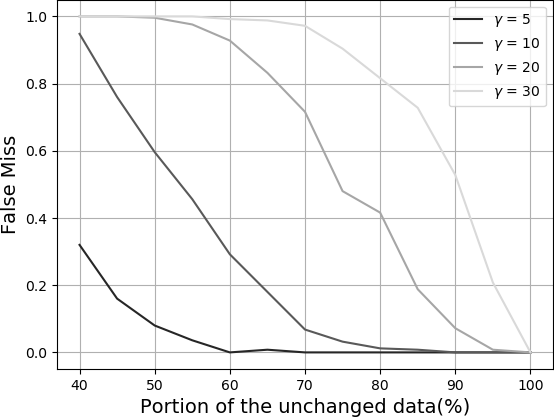
\includegraphics[width=1\linewidth]{figures/bit-flipping_n_grey.png}
        \caption{Nursery dataset}
        \label{fig:bit-flipping-n}
    \end{subfigure}
    \caption{Robustness against flipping attack}
    \label{fig:bit-flipping}
\end{figure*}

We show the results of the flipping attack simulation in \Cref{fig:bit-flipping-bc} and \Cref{fig:bit-flipping-n}. The false miss rate is recorded in dependence on the percentage of data values \textit{not} affected by the attacker. 
The false miss rate is generally bigger if the attacker altered more data. 
We show the results for 40\% and more unchanged values. 
Modifying more than 60\% of the data values seriously affects the dataset credibility, therefore we assume such data is not usable.
The most robust scheme for Breast Cancer is again the scheme with $\gamma=1$; false miss rate measured on datasets with 40\% of unchanged(original) values is about 0.1.
The scheme for Nursery data with $\gamma=5$ is very robust against a flipping attack; the false miss rate is close to zero in most of the experiments. On the other hand, schemes with larger $\gamma$ values, $\gamma=20$ and $\gamma=30$, show much poorer robustness results.

\subsection{Data Utility Effects}\label{sec:utility}
In the previous section we showed that better robustness of the scheme is achieved by embedding more marks into the data. 
However, more marks imply more alterations and reduction of data quality and utility, e.g. for the data mining tasks we want to perform on the data.

We thus measure utility of the fingerprinted data. To this end, we compare the performance of a predictive classifier trained with that data, to one trained on the original, not modified dataset. 
\begin{table}[ht]
    \centering
    \caption{Parameter settings}
    \begin{tabular}{@{}l|llll@{}}
     \toprule
         & Decision & Logistic  &  & Gradient\\
         & Tree & Regression & k-NN & Boosting \\
         \midrule
         Breast & \textbf{max\_depth}: 2 & \textbf{solver}: 'saga' & \textbf{n\_neighbors}: 19 & \textbf{n\_estimators}: 200 \\
         Cancer & \textbf{criterion}: 'entropy' & \textbf{C}: 90 &  \textbf{algorithm}: 'kd\_tree' & \textbf{loss}: 'exponential'\\
         &&&& \textbf{criterion}: 'mae'\\
         \hline
         &\textbf{max\_depth}: 13 & \textbf{solver}: 'lbfgs' & \textbf{n\_neighbors}: 8 & \textbf{n\_estimators}: 100 \\
        Nursery & \textbf{criterion}: 'entropy' & \textbf{C}: 20 &  \textbf{algorithm}: 'kd\_tree' & \textbf{loss}: 'deviance' \\
        &&&& \textbf{criterion}: 'friedman\_mse'\\
        \bottomrule
    \end{tabular}
    \label{tab:parameter-setting}
\end{table}

Specifically, we measure the micro-averaged classification accuracy, which is the percentage of correctly classified data samples, using a 10-fold cross-validation. 
The classification accuracy is measured in the interval [0,100]\%.
We use the following classification models:
Decision Tree, Logistic Regression, k Nearest Neighbours (k-NN) and Gradient Boosting, with the hyper-parameter settings in \Cref{tab:parameter-setting} obtained from a random search with 10 iterations over the following search domain\footnote{Other parameters are set to default values from the \textit{scikit-learn} Python library}:
\begin{itemize}
    \item Decision Tree: \textbf{max\_depth}:(1, 30), \textbf{criterion}:['gini', 'entropy']
    \item Logistic Regression: \textbf{solver}:['liblinear', 'newton-cg', 'lbfgs', 'saga'], \textbf{C}:(10, 100)
    \item k-NN: \textbf{n\_neighbors}:(1, 20), \textbf{algorithm}:['auto', 'ball\_tree', 'kd\_tree', 'brute']
    \item Gradient Boosting: \textbf{n\_estimators}:(50, 200), \textbf{loss}:['deviance', 'exponential'], \textbf{criterion}:['friedman\_mse', 'mse', 'mae']
\end{itemize}

For each of the models, we first obtained the result on the original dataset (equivalent to $\gamma$=0).
We then trained the models on the fingerprinted datasets, using the same hyper-parameters.
For clarity of the results, we report the \textit{differences in classification accuracy} when training these two settings.


\begin{table}[ht]
\centering
\caption{Impact on classification accuracy on the Breast Cancer dataset}
\label{tab:ml-breast-cancer}
\begin{tabular}{@{}c|cccc@{}}
\toprule
$\gamma$ & \multicolumn{1}{c}{Decision Tree} & \multicolumn{1}{c}{Logistic Regression} & \multicolumn{1}{c}{k-NN} & \multicolumn{1}{c}{Gradient Boosting} \\ \midrule
0 & \textcolor{blue}{71.68\%} & \textcolor{blue}{66.78\%} & \textcolor{blue}{75.17\%} & \textcolor{blue}{67.83\%} \\
\hline
1     & -3.15\%                           & -0.15\%                                 & -1.86\%                 & -1.14\%                              \\
2     & -1.75\%                           & -0.08\%                                 & -1.29\%                  &    -0.40\%                                   \\
3     & -5.24\%                           & -0.70\%                                 & -1.18\%                  &  -0.61\%
\\
5     & -1.74\%                           & -0.35\%                                 & -0.77\%                  & -0.30\%                               \\ \bottomrule
\end{tabular}
\end{table}

\Cref{tab:ml-breast-cancer} shows the results for the Breast Cancer dataset.
We can observe that there is a general trend that the lower the value is for $\gamma$, the lower is also the impact on the classification accuracy, though the trend is not linear, and some deviations from this trend occur for specific settings.
Specifically Logistic Regression is affected only marginally. While Decision Trees show a larger degradation, k-NN and even better Gradient Boosting are not degrading significantly.

\begin{table}[h]
\centering
\caption{Impact on classification accuracy on the Nursery dataset}
\label{tab:ml-nursery}
\begin{tabular}{@{}c|cccc@{}}
\toprule
$\gamma$ & Decision Tree & Logistic Regression & k-NN    & Gradient Boosting \\ \midrule
0 & \textcolor{blue}{77.99\%} & \textcolor{blue}{84.50\%} & \textcolor{blue}{77.30\%} & \textcolor{blue}{98.38\%} \\
\hline
1 & -1.84\% & -2.22\% & -2.94\% & -5.82\% \\
3 & -0.66\% & -0.78\% & -1.02\% & -2.05\% \\
5     & -0.85\%       & -0.42\%             & -0.41\% & -1.30\%           \\
10    & -0.59\%       & -0.21\%             & -0.21\% & -0.64\%           \\
20    & -0.83\%       & -0.10\%             & -0.10\% & -0.33\%           \\
30    & -0.40\%       & -0.08\%             & -0.18\% & -0.25\%           \\ \bottomrule
\end{tabular}
\end{table}

In \Cref{tab:ml-nursery}, we see that the general trend, i.e. that the impact on the classification accuracy is lower for bigger $\gamma$, is present in the Nursery dataset as well. 
%The overall loss in classification accuracy is much smaller than in the Breast Cancer dataset.
%The choice of larger values for $\gamma$ affects these results.  
We can see that the loss in accuracy for $\gamma=1$ and $\gamma=3$ is significantly bigger compared to other cases and is in the same magnitude as the results with Breast Cancer data and the same $\gamma$ values. However, in this case with the low $\gamma$ values, Gradient Boosting is the worst classifier, and Logistic Regression has a significantly higher degradation for small $\gamma$ values than on the Breast Cancer dataset.
For higher values of $\gamma$, Decision Trees and Gradient Boosting are affected the most. Logistic Regression and k-NN show a smaller degradation in this case.

Overall, the choice of the parameter $\gamma$ should lean towards larger values because the impact on the classification accuracy is in that case lower.
However, an acceptable trade-off with the desired robustness settings needs to be found.

\section{Conclusion and Future Work}\label{sec:conclusion&future-work}
We present a novel scheme for fingerprinting categorical attributes in relational databases.
The scheme is designed such that it minimises the occurrence of non-existing and rare combinations of values in the fingerprinted dataset, preserving that way the semantic coherence of the dataset.
Furthermore, we presented two types of analysis for our scheme: (i) robustness analysis that measures scheme's vulnerability to malicious attacks, and (ii) the data utility analysis that measures the effects that the fingerprint has on a classification accuracy.

The most important parameter $\gamma$, defining the amount of marks in the data, has a dual effect on the scheme. We showed in \Cref{sec:robustness} that a smaller $\gamma$ values make the scheme more robust against all types of mentioned attacks.
On the other hand, the analysis in \Cref{sec:utility} shows that smaller $\gamma$ values lead to larger effect on the data classification accuracy. 
Therefore, $\gamma$ should be selected in a trade-off between scheme's robustness and data utility. 

Future work will be focused towards designing a scheme that unifies the processes of fingerprinting different types of data and, therefore, enhance the applicability of fingerprinting to real-life, mixed-type relational datasets.

%TODO: we forgot this in the initial version, we need to make some more space for it :-)
\section*{Acknowledgement}
This work was partially funded by the EU Horizon 2020 research and innovation programme under grant agreement No 732907 
% project name can be skipped if needed
(project ``MyHealthMyData'') 
and the ``Industrienahe Dissertationen'' program (No 878786) of the Austrian Research Promotion Agency (FFG)
%full name
%(project ``Intellectual Property Protection for Machine Learning Processes'')
% or just use short name
 (project ``IPP4ML'')

%
% ---- Bibliography ----
%
% BibTeX users should specify bibliography style 'splncs04'.
% References will then be sorted and formatted in the correct style.
%
\bibliographystyle{unsrt}
\bibliography{biblio}
%
\end{document}
